\documentclass{gost}

%-------------------------------------------------------------------------------
%
% ПЕРЕМЕННЫЕ
%
%-------------------------------------------------------------------------------

\newcommand{\universityFullName}{Федеральное государственное бюджетное
образовательное учреждение высшего образования Саратовский Государственный
Технический Университет имени Гагарина Ю.А.}
\newcommand{\universityShortName}{СГТУ им. Гагарина Ю.А.}
\newcommand{\department}{Прикладные информационные технологии}
\newcommand{\nirName}{Лабораторная работа по выбору и установке операционной
системы}
\newcommand{\nirType}{промежуточный}
\newcommand{\nirStage}{1}
\newcommand{\subject}{Программные и аппаратные технологии умного города}

%-------------------------------------------------------------------------------
%
% ДОКУМЕНТ
%
%-------------------------------------------------------------------------------

\begin{document}
	\gostTitlePage

	\section{Задачи}
		\begin{enumerate}
			\item Настроить виртуальную машину.
			\item Спланировать установку виртуальной машины.
			\item Установить порядок загрузки машины.
			\item Разметить диск для установки ОС.
			\item Установить ОС и получить доступ к ее командной оболочке.
		\end{enumerate}

	\section{Выполнение задачи №1}
		В качестве основной ОС я использую Arch Linux, поэтому установка виртуальной
		машины будет выглядеть следующим образом.

		\begin{figure}[H]
			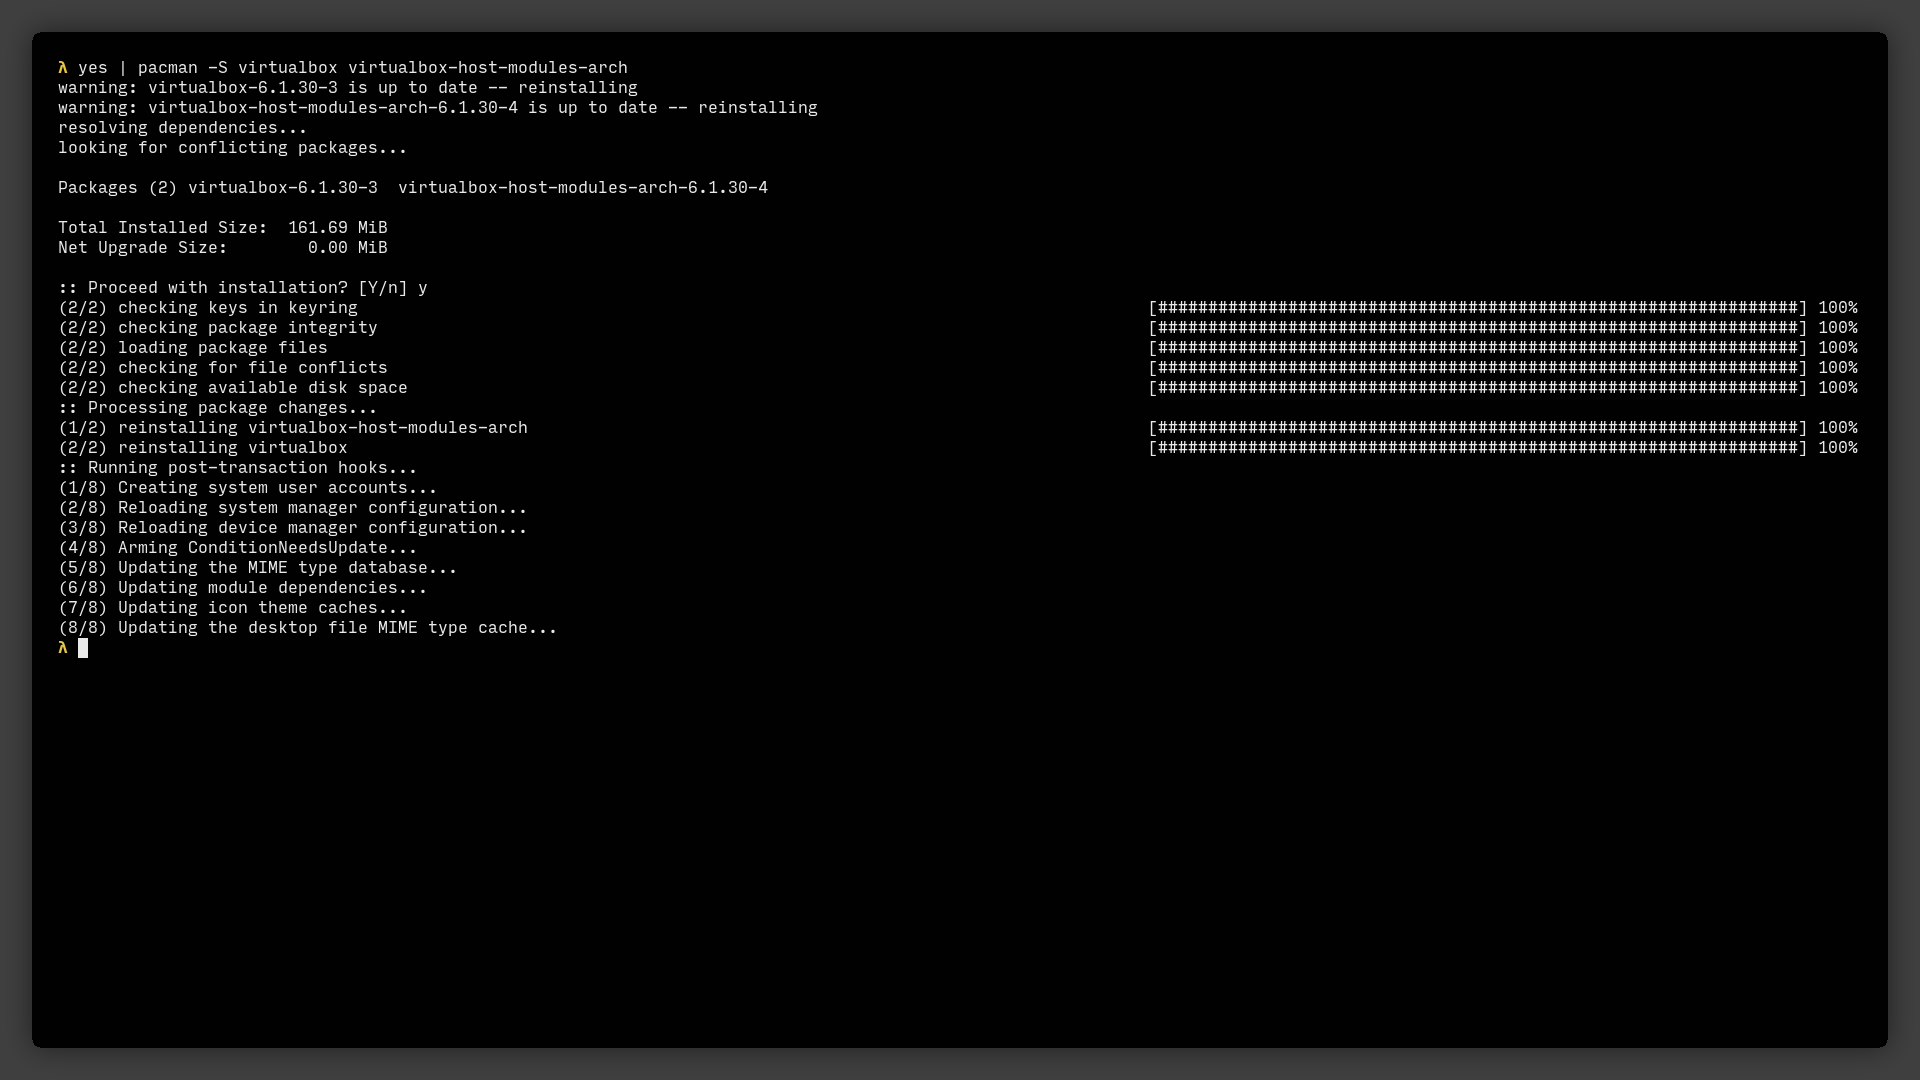
\includegraphics[width=\textwidth,clip=true]{img/1.png}
			\caption{Установка Oracle® VirtualBox в Arch Linux}
		\end{figure}

	\section{Выполнение задачи №2}
		Создаем новую вирутальную машину под названием \enquote{Arch Linux}. В итоге
		получаем следующую картину:

		\begin{figure}[H]
			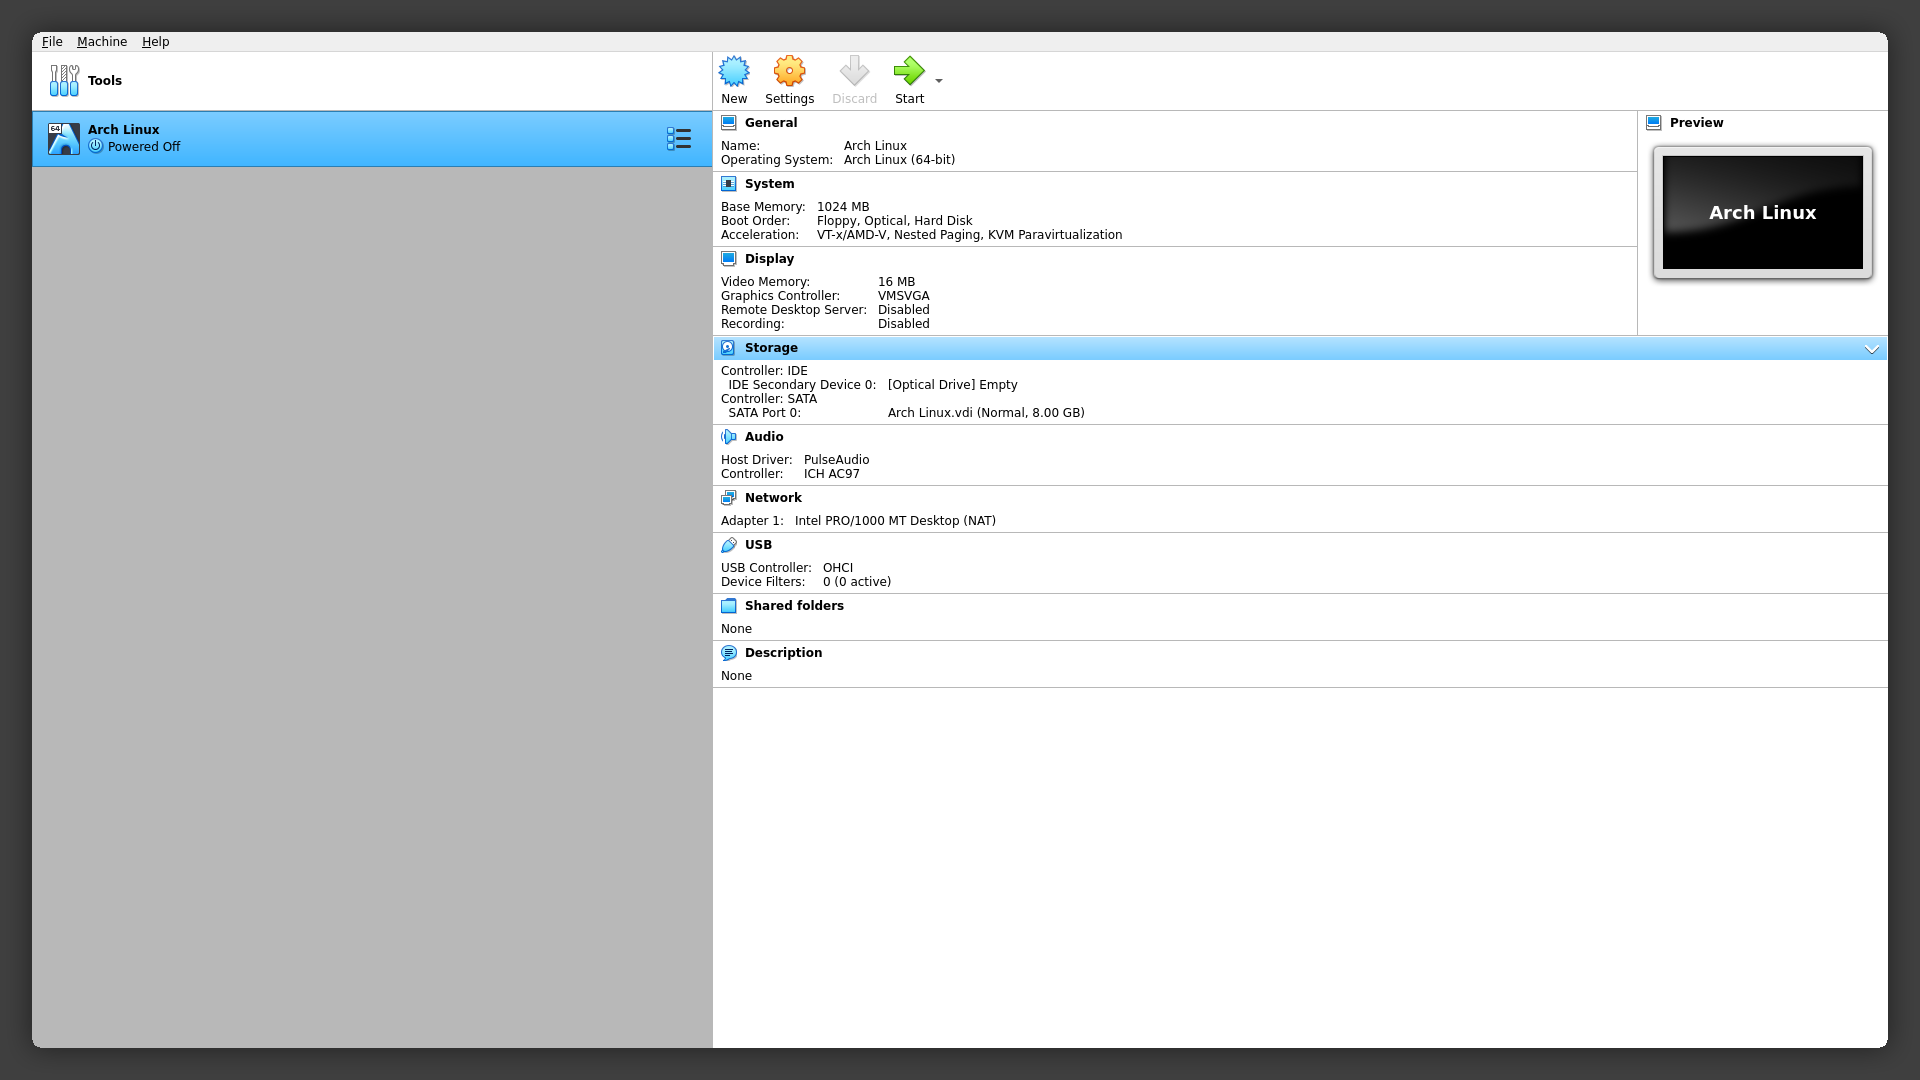
\includegraphics[width=\textwidth,clip=true]{img/2.png}
			\caption{Создали новую виртуальную машину под названием Arch Linux}
		\end{figure}

	\section{Выполнение задачи №3}
		Теперь вставляем в CD-ROM только что созданной виртуальной машины ISO-образ
		операционной системы Arch Linux и устанавливаем порядок загрузки.

		\begin{figure}[H]
			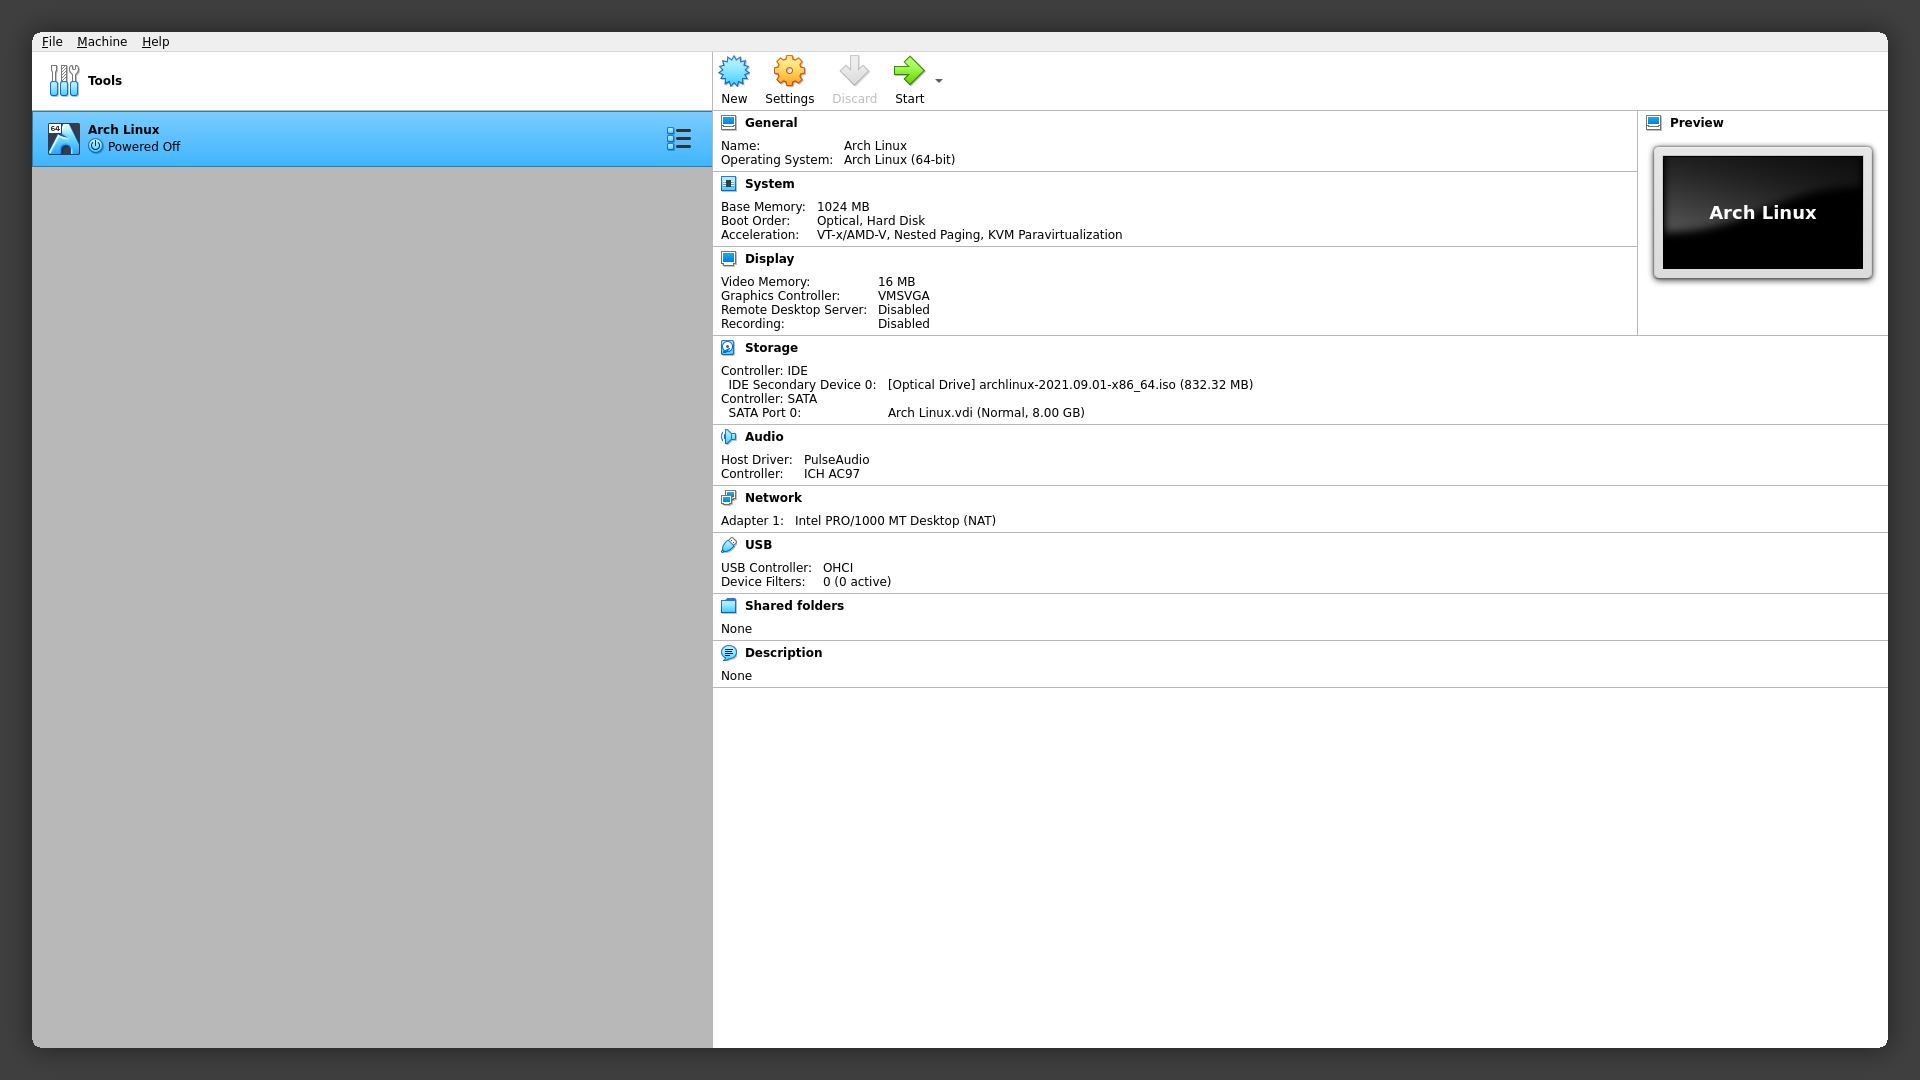
\includegraphics[width=\textwidth,clip=true]{img/3.png}
			\caption{Виртуальная машина со вставленым в CD-ROM ISO-образом и нужным
			приоритетом загрузки}
		\end{figure}

	\section{Выполнение задачи №4}
		Размечаем диск для установки ОС с помощью программы GNU Parted.

		\begin{figure}[H]
			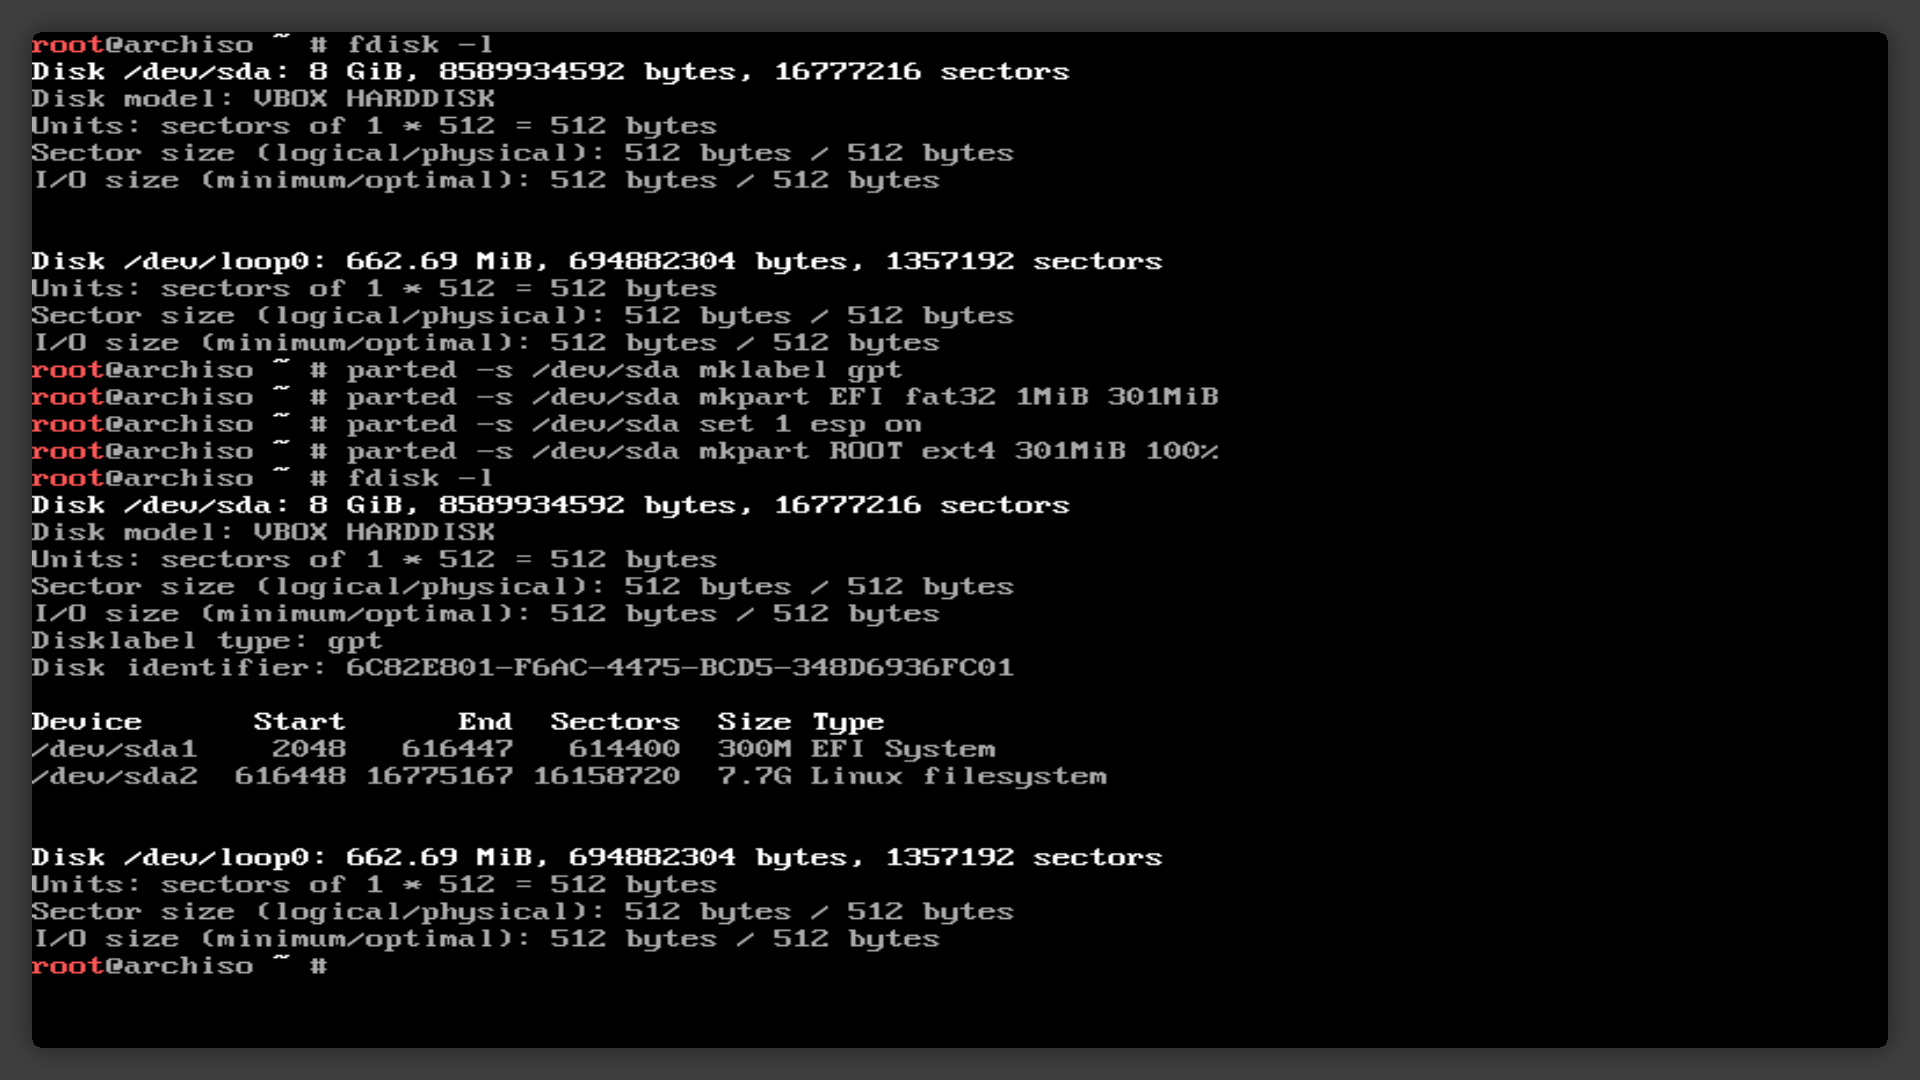
\includegraphics[width=\textwidth,clip=true]{img/4.png}
			\caption{Процесс разметки диска для установки ОС и результат разметки}
		\end{figure}

	\section{Выполнение задачи №5}
		Далее мы устанавливаем ОС по инструкции на Arch Wiki. В итоге получаем
		установленную ОС и доступ к её командной оболочке:

		\begin{figure}[H]
			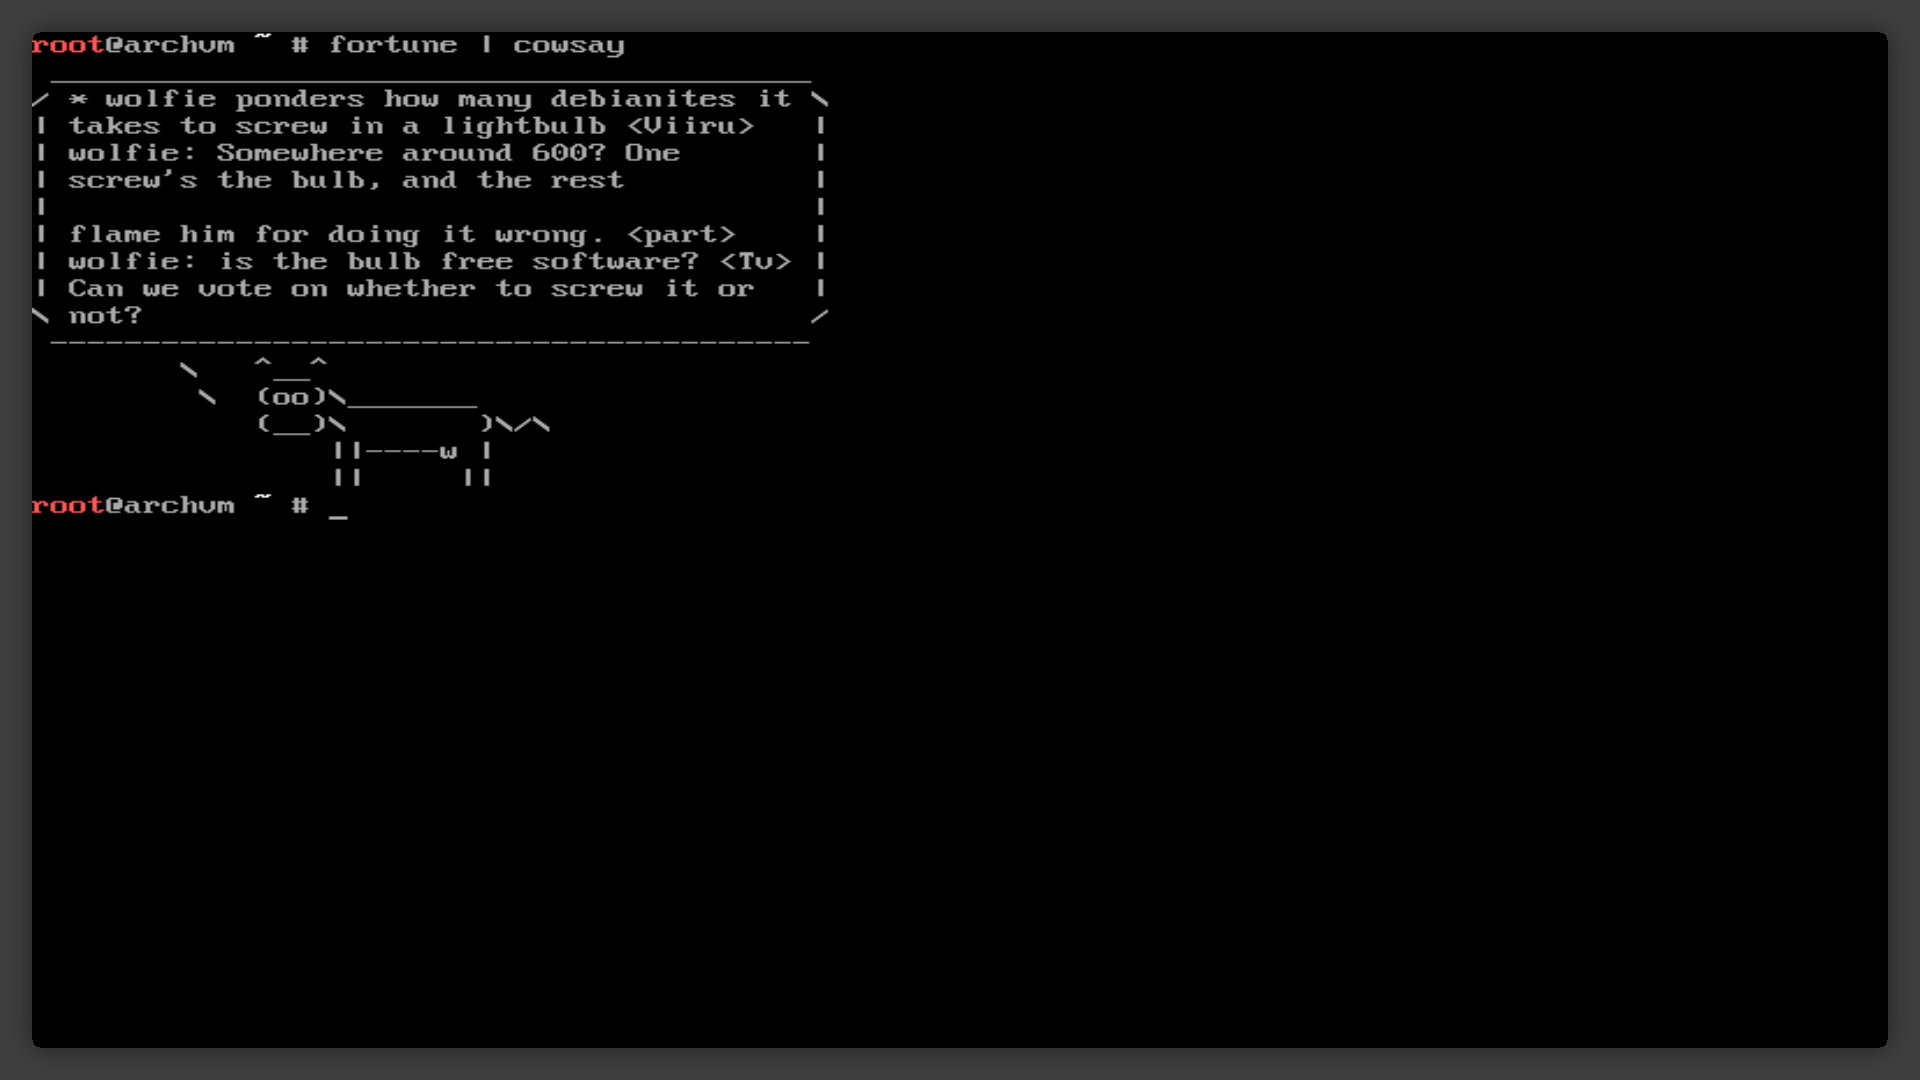
\includegraphics[width=\textwidth,clip=true]{img/5.png}
			\caption{Вызов программ из командной оболочки zsh свежеустановленной ОС}
		\end{figure}
\end{document}
